---
title: Causal Directed Acylic Graphs
subtitle: introduction
author: Wouter van Amsterdam
date: 2024-08-06
format: 
    #latex:
        #documentclass: beamer
        #lof: true
        #lot: true
    #html:
        #toc: true
        #toc-depth: 2
        #number-sections: true
    revealjs:
        theme: umcu.scss
        incremental: true
        width: 1600
        height: 900
        logo: umcu_blue.png
        center: true
execute:
    warning: false
    message: false
categories:
    - DAG
    - day2
bibliography: bibliography.bib
filters:
    - diagram
diagram:
  cache: true
  engine:
    tikz:
      execpath: lualatex
      header-includes:
        - '\usepackage{adjustbox}'
        - '\usetikzlibrary{arrows, shapes, positioning}'
        - '\tikzstyle{nodeobserved} = [circle, minimum size = 10mm, thick, draw =black!80, fill=gray!30]'
---
---

```{r}
#| label: setup
#| echo: false
#| execute: true

suppressMessages({
  library(purrr)
  library(data.table)
  library(ggplot2); theme_set(theme_bw())
  library(knitr)
})
```


<!--

Qs:

1. what knowledge of probability to expect? e.g. conditioning

--->

## Causal inference frameworks

### What are they for?

#### Mathematical language to
  - define *causal* quantities
  - express *assumptions*
  - derive how to *estimate* causal effects

## Causal inference frameworks

### Why learn more than one?

<!--todo: add hyperlink to day 1 materials-->

- On day 1 we learned about the Potential Outcomes framework
    - Defines causal effects in terms of (averages of) *individual potential outcomes*
    - Estimation requires assumptions of (conditional) exchangeability and positivity / overlap and consistency
- There isn't only 1 way to think about causality, find one that '*clicks*'
- Now we will learn another framework: *structural causal models* (SCMs)
    - SCM approach is broader in that it can define more different types of causal questions
- Equivalence: given the same data and assumptions, get the same estimates

## lecture 1 topics

- why are DAGs useful
- what are DAGs and where do come from 
- SCMs as computer programs
  - intervention as change in program
- causal identifyability with DAGs
  - variable types: confounders, mediators, colliders (tinder: hot and intelligent / single ;on tinder)
    - confounders; storks; randomized, breaking arrows
  - d-separation
  - back-door criterion
  - follow rules of do calculus


-  DAG
  1. what is the world
  2. what can we estimate and how?
  3. confounders / colliders
  4. backdoor
 
## lecture 2 topics

  - perfect versus soft intervention
  - critique of scm / cross-world assumptions

## practical 1

  - drawing and using dags (what to condition on); daggity
  - same data, different dags, different answers

## lecture 3 topics

  - bonus queries:
    - counterfactuals
    - probability of necessity, probability of sufficiency
    - actual causality (Joe Halpern)
  - Pearl Causal Hierarchy
  - other uses of DAGs: missing data, selection
  - reflections on DAGs, limitations

## practical 2

  - causal ladder: what Q is this?
  - give data of hierarchy and answer the Q
  - give data of 2 treatments + SCM (treatment 3 which can be extrapolated from)

# Why are DAGs useful

## Example task: are hospital deliveries good for babies?

::: {.r-stack}

![](figs/delivery1.png)

![](figs/delivery2.png){.fragment}

![](figs/delivery.png){.fragment}

:::

## Example task: are hospital deliveries good for babies?

- You're a data scientist in the Wilhelmina Kinderziekenhuis (WKZ)
- Have data on
  - delivery location (home or hospital)
  - neonatal outcomes (good or bad)
  - pregnancy risk (high or low)
- Question: do hospital deliveries result in better outcomes for babies?

. . .

```{r}
#| label: simdeliveries

# t=0: home, t=1: hospital
# z=0: low risk, z=1: high risk
# y=1: good outcome
dnames = list(location=c('home', 'hospital'), risk=c('low', 'high'))
pos_tz <- matrix(c(
  c(0.9,  0.5), # y|t=0,z=0,1
  c(0.95, 0.8)  # y|t=1,z=0,1
), nrow=2, byrow=T,
dimnames=dnames)

ps_tz <- matrix(c(
  c(0.72, 0.08), # p(t=0,z=0,1)
  c(0.02, 0.18)  # p(t=1,z=0,1)
), nrow=2, byrow=T, dimnames=dnames)

# p(t,z) under do(t)
ps_do0 <- matrix(c( 
  c(0.8, 0.2), 
  c(0.0, 0.0)  
), nrow=2, byrow=T)

ps_do1 <- matrix(c( 
  c(0.0, 0.0), 
  c(0.8, 0.2) 
), nrow=2, byrow=T)


eys  <- rowSums(pos_tz * ps_tz) / rowSums(ps_tz) # E y|t
dots <- c(sum(pos_tz * ps_do0), sum(pos_tz*ps_do1))

n = 1000

ts  <- vector(mode="logical", length=0)
zs  <- vector(mode="logical", length=0)
py0s <- vector(mode="numeric", length=0)
py1s <- vector(mode="numeric", length=0)
ys  <- vector(mode="logical", length=0)

ntots <- n * ps_tz

for (t in c(0,1)) {
  for (z in c(0,1)) {
    ntz <- n *ps_tz[t+1,z+1]
    ts  <- c(ts, rep(t, ntz))
    zs  <- c(zs, rep(z, ntz))
    py <- pos_tz[t+1,z+1]
    y <- c(rep(0,
               round(ntz * (1-py))), # <- round should not be needed here but found a bug
           rep(1,
               round(ntz*py))) 
    ys <- c(ys, y)
    py0s <- c(py0s, rep(pos_tz[1, z+1], ntz))
    py1s <- c(py1s, rep(pos_tz[2, z+1], ntz))
  }
}
# ys <- ifelse(ts, y1s, y0s)
df <- data.table(
  location=ts,
  risk=zs,
  outcome=ys,
  py0=py0s,
  py1=py1s)

# head(df)

# kable(eys, col.names="tips")
#pander::pander(ftable(eys))

# pander::pander(ftable(pos_tz), emphasize.strong.rows=c(1), emphasize.strong.cols=c(1))

ntots <- n * ps_tz
nys <- ntots * pos_tz

strs <- paste0(nys, " / ", ntots, " = ", 100*pos_tz, "%")
str_mat <- matrix(strs, ncol=2, dimnames=dnames)
# kable(t(str_mat))
# pander::pander(ftable(t(str_mat)), emphasize.strong.rows=c(1), emphasize.strong.cols=c(1))

ntotsm <- rowSums(ntots)
nysm <- rowSums(nys)
strsm <- paste0(nysm, " / ", ntotsm, " = ", 100*eys, "%")

tab_tots <- rbind(ntots, ntotsm)


# tab <- df[, list(good=sum(outcome==1), bad=sum(outcome==0), frac_good=mean(outcome)), by=c("risk", "location")]


```

. . . 


```{r}
#| label: deliveryplot
#| output: fragment
#| include: false

df[, ni:=1.]

ggplot(df, aes(x=1, fill=factor(outcome))) +
  geom_bar(stat="count", position="stack") + 
  # geom_bar(aes(y=..count../sum(..count..))) + 
  facet_grid(risk~location)
```


## Observed data {auto-animate=true}

|      |      | location |          |
|------|------|---------:|---------:|
|      |      | home     | hospital |
| risk | low  | `r str_mat[1,1]` | `r str_mat[2,1]` |
|      | high | `r str_mat[1,2]` | `r str_mat[2,2]` |


## Observed data {auto-animate=true}

|      |      | location |          |
|------|------|---------:|---------:|
|      |      | home     | hospital |
| risk | low  | `r str_mat[1,1]` | `r str_mat[2,1]` |
|      | high | `r str_mat[1,2]` | `r str_mat[2,2]` |
|      |      |                  |                  |
|      | *marginal* | `r strsm[1]` | `r strsm[2]` |

- better outcomes for babies delivered in the hospital for *both risk groups*
- but not better *overall*
- how is this possible? (a.k.a. *simpsons paradox*)
- what is the correct way to estimate the effect of delivery location?

## New question: can a patient walk 1 week after getting a hernia?

::: {.r-stack}

![](figs/delivery-locations.png){.fragment}

![](figs/delivery-backpain.png){.fragment}

:::

## Observed data 2

|      |      | location |          |
|------|------|---------:|---------:|
|      |      | home     | hospital |
| bedrest | no | `r str_mat[1,1]` | `r str_mat[2,1]` |
|      | yes | `r str_mat[1,2]` | `r str_mat[2,2]` |
|      |      |                  |                  |
|      | *marginal* | `r strsm[1]` | `r strsm[2]` |

- more bed rest in hospital
- what is the correct way to estimate the effect of location?

## How to unravel this?

- we got two questions with exactly the same data
- in one example, 'stratified analysis' seemed best
- in the other example, 'marginal analysis' seemed best
- with *Directed Acyclic Graphs* we can make our decision

## DAGs

1. nodes are variables
2. arrows point from cause to effect

::: {layout-ncol=2}

:::: {#fig-dag-delivery .fragment}

``` {.tikz}
%%| filename: dag-delivery.pdf

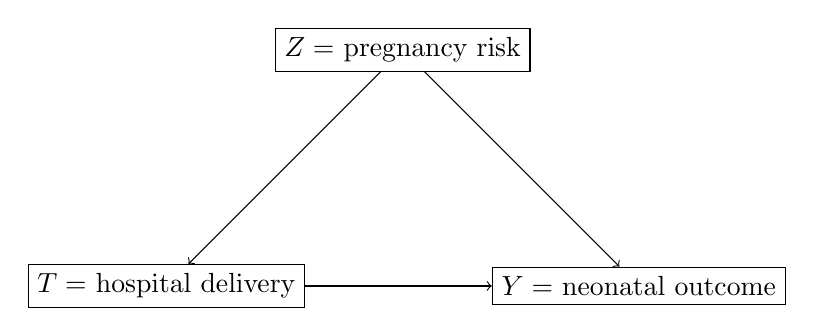
\begin{tikzpicture}
  % Nodes
  \node[draw] (z) at (0, 3) {$Z=$ pregnancy risk};
  \node[draw] (t) at (-3, 0) {$T=$ hospital delivery};
  \node[draw] (y) at (3, 0) {$Y=$ neonatal outcome};

  % Edges
  \draw[->] (z) -- (t);
  \draw[->] (z) -- (y);
  \draw[->] (t) -- (y);

\end{tikzpicture}
```

::::

:::: {#fig-dag-hernia .fragment}

``` {.tikz}
%%| filename: dag-hernia.pdf

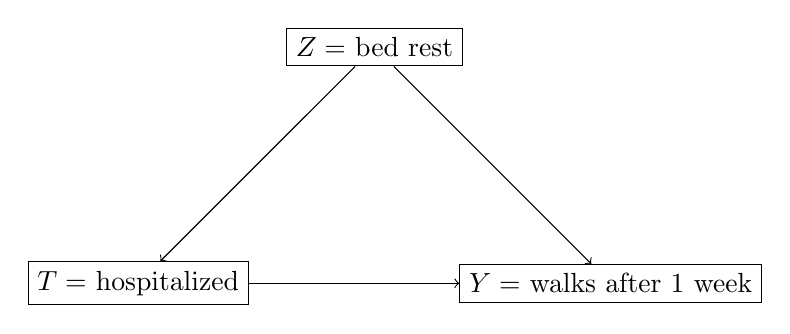
\begin{tikzpicture}
  % Nodes
  \node[draw] (z) at (0, 3) {$Z=$ bed rest};
  \node[draw] (t) at (-3, 0) {$T=$ hospitalized};
  \node[draw] (y) at (3, 0) {$Y=$ walks after 1 week};

  % Edges
  \draw[->] (z) -- (t);
  \draw[->] (z) -- (y);
  \draw[->] (t) -- (y);

\end{tikzpicture}
```

::::

:::

## tikz example

::: {#fig-dag}


``` {.tikz}
%%| label: dag1
%%| fig-align: "center"
%%| filename: dag1.pdf
%%| alt: DAG 1

\resizebox{16cm}{!}{%
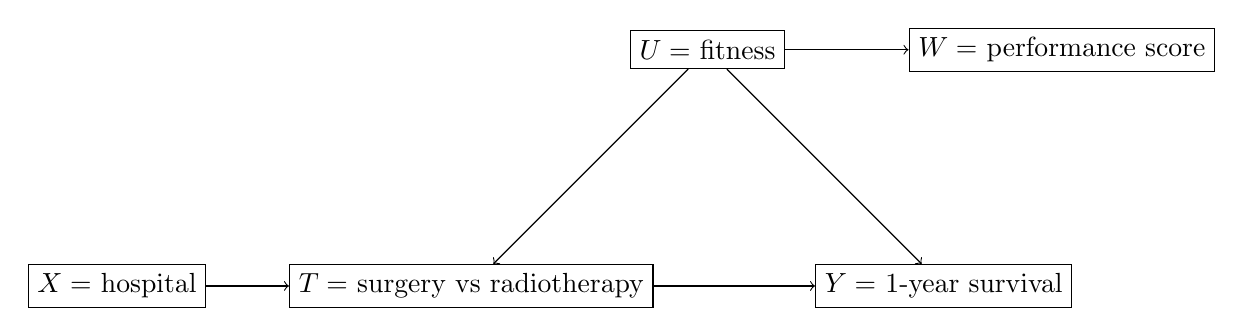
\begin{tikzpicture}
		  % Nodes
		\node[draw] (z) at (0, 3) {$U=$ fitness};
		  \node[draw] (t) at (-3, 0) {$T=$ surgery vs radiotherapy};
		  \node[draw] (y) at (3, 0) {$Y=$ 1-year survival};
          \node[draw] (x) at (-7.5,0) {$X=$ hospital};
		  \node[draw] (w) at (4.5,3) {$W=$ performance score};

		  % Edges
		  \draw[->] (z) -- (t);
		  \draw[->] (z) -- (y);
		  \draw[->] (t) -- (y);
          \draw[->] (z) -- (w);
          \draw[->] (x) -- (t);
\end{tikzpicture}
}

```

:::

## DAGs are non-parametric

::: {layout="[70,30]" layout-valign="center"}

```{r}
#| label: fig-dag-nonparametric
#| output: fragment
#| fig-cap: Three datasets with the same DAG

set.seed(12345)
n = 1e3

f1 <- function(t, x, u) t + 0.5 * (x - pi) + u
f2 <- function(t, x, u) t + sin(x) + u
f3 <- function(t, x, u) t * sin(x) - (1-t) * sin(x) + u

df <- data.table(
  x = runif(n, 0, 2*pi),
  t = rbinom(n, 1, 0.5),
  u = rnorm(n, 0, .1)
)
df[, `:=`(
  y1 = f1(t, x, u),
  y2 = f2(t, x, u),
  y3 = f3(t, x, u)
)]

dfm <- melt(df, measure.vars=c('y1', 'y2', 'y3'),
            variable.name="f", value.name="y")

ggplot(dfm, aes(x=x, y=y, col=factor(t))) + 
  geom_point() + 
  facet_grid(~f)

```

``` {.tikz}
%%| filename: dag-nonparametric.pdf
%%| fig-align: "center"

\scalebox{3}{
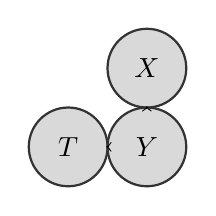
\begin{tikzpicture}
  % Nodes
  \node[nodeobserved] (z) at (0, 1) {$X$};
  \node[nodeobserved] (t) at (-1, 0) {$T$};
  \node[nodeobserved] (y) at (0, 0) {$Y$};

  % Edges
  \draw[->] (z) -- (y);
  \draw[->] (t) -- (y);

\end{tikzpicture}
}
```

:::

## next steps


*conclusion 1*: seeing is not doing

**to follow-up**

- DAG to picture the game
- doing = mutilating DAG
- hotel 2: the Randtz
- identifyability: more SCMs with same marginals
- another hidden variable: are the guests brittish
- SCM = know rules of the game
- DAG = know who listens to what
- why are DAGs useful? know what you can compute



## References

